% !TEX root = Network.tex



%% Type de document et encodage de la police
\documentclass[a4paper]{article}
\usepackage[utf8x]{inputenc}
\usepackage[T1]{fontenc}
% \usepackage[french]{babel}

%% Initialise la taille des pages et des marges
\usepackage[a4paper, top=3cm, bottom=3cm, left=2cm, right=2cm, marginparwidth=2cm]{geometry}

%% Packs utiles
\usepackage{amsmath}
\usepackage{xcolor}

%% Commandes perso
\renewcommand{\tt}{\texttt}
\renewcommand{\contentsname}{Table des Matières}
\renewcommand{\arraystretch}{1.5} %% row 50% longer
\definecolor{sprinen}{rgb}{0.0, 1.0, 0.7}

%% Pour les exemples
\usepackage{mdframed}
\newmdenv[topline=false, bottomline=false, rightline=false, skipabove=\topsep, skipbelow=\topsep]{example}

%% Pour les diagrammes
\usepackage{tikz}
\usetikzlibrary{shapes.geometric, calc, arrows}
\tikzstyle{incolore} = [rectangle, rounded corners, draw=black, minimum height=1cm, minimum width=3cm, text width=3cm, text centered]

%% import tex documents
\usepackage[subpreambles=true]{standalone}
\usepackage{import}


\title{Réseaux Applicatifs - Labos}
\author{Grégoire Roumache}
\date{Octobre 2019}

\begin{document}

\maketitle

\tableofcontents















\textcolor{red}{\section{Attention !}}

\begin{itemize}
    \item La partie \textbf{Wireshark} ne contient qu'une liste de filtres. Voir le labo sur Wireshark pour l'utilisation du logiciel.
\end{itemize}















\section{Changer la configuration via la ligne de commande}










\subsection{Windows}





\begin{example}
    Ouvrir l'invite de commande en tant qu'administrateur.    
\end{example}





\begin{itemize}





%% Mode Statique -- Windows CLI
\item Passer en mode statique:
\begin{enumerate}
    \item Noter les paramètres réseaux: \tt{ipconfig /all}.
    \item Désactiver le DHCP (2 possibilités): \\
    \tt{netsh interface ip add address "Ethernet" <adr\_ip> <netmask> [<def\_gateway>]} \\
    \tt{netsh interface ip set address "Ethernet" static <adr\_ip> <netmask> [<def\_gateway>]}
\end{enumerate}

\begin{center} \textcolor{blue}{\textbf{Attention ! Si on veut tester la connexion à [1.1.1.1] avec ping, il faut avoir mis un default gateway.}} \end{center}





%% Mode Dynamique -- Windows CLI
\item Passer en mode dynamique:
\begin{enumerate}
    \item Ré-activer le DHCP avec: \tt{netsh interface ip set address "Ethernet" dhcp}.
    \item Vérifier si le DHCP est bien activé: \tt{ipconfig /all}.
\end{enumerate}





%% Ping Réseau Interne -- Windows CLI
\item Ping dans un réseau interne:
\begin{center}
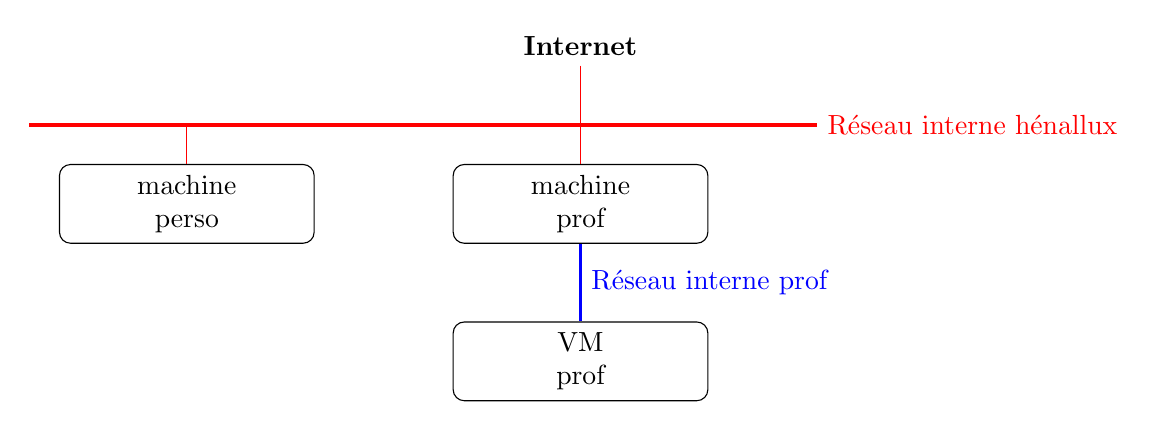
\begin{tikzpicture}
    %% réseau interne henallux
    \draw[-, very thick, red] (0,0) -- (10,0) node[anchor=west]{Réseau interne hénallux};

    %% machine perso
    \node (perso) [incolore] at (2,-1) {machine \\perso};
    \draw[-, red] (perso) -- (2,0);

    %% internet
    \node (internet) [] at (7,1) {\textbf{Internet}};
    \draw[-, red] (internet) -- (7,0);

    %% machine prof
    \node (prof) [incolore] at (7,-1) {machine \\prof};
    \draw[-, red] (prof) -- (7,0);

    %% VM prof
    \node (VMprof) [incolore] at (7,-3) {VM \\ prof};
    \draw[-, very thick, blue] (prof) -- node[anchor=west]{Réseau interne prof} (VMprof);
\end{tikzpicture}
\end{center}

Imaginons qu'on ait la configuration suivante:
\begin{itemize}
    \item machine prof = 10.101.101.189
    \item réseau interne prof = 172.16.10.0
    \item netmask = 255.255.255.0
    \item VM prof = 172.16.10.20
\end{itemize}
il faut utiliser la commande \texttt{route add} pour ajouter un default gateway:
\begin{center} \begin{tabular}{ccccc}
route add & <network> & mask & <netmask> & <default\_gateway> \\
route add & 172.16.10.0 & mask & 255.255.255.0 & 10.101.101.189
\end{tabular} \end{center}

\begin{center}
\textcolor{blue}{\textbf{Remarque: il faut avoir désactivé le firewall (voir configuration via GUI -- section \ref{subsec:WindowsGUI}).}}
\end{center}

\end{itemize}










\subsection{Linux} \label{subsec:LinuxCLI}





\begin{example}
    Clavier belge: \tt{setxkbmap be}. \\
    Super-utilisateur: \tt{su - root}.
\end{example}





\begin{itemize}





%% Mode Statique -- Debian CLI
\item Passer en mode statique:
\begin{enumerate}
    \item Noter les paramètres réseaux: \tt{ip a}.
    \item Désactiver le DHCP: \tt{ip addr flush dev <interface\_réseau>}
    \item Ajouter une adresse IP: \tt{ip addr add <adresse\_ip>/<netmask> dev <interface>}
    \begin{example}
        ex: \tt{ip addr add 192.168.30.20/24 dev enp0s3}
    \end{example}
\end{enumerate}
\textcolor{blue}{\textbf{Remarque: impossible de ping [1.1.1.1] si on ne met pas /24 après l'ip.}}





%% Mode Dynamique -- Debian CLI
\item Passer en mode dynamique:
\begin{enumerate}
    \item Ré-activer le DHCP avec: \tt{dhclient -v <interface>}.
    \item Afficher les process DHCP: \tt{ps aux | grep dhclient}.
\end{enumerate}





%% Ping Réseau Interne -- Linux CLI
\item Ping dans un réseau interne: dans la situation suivante,
\begin{itemize}
    \item machine prof = 10.101.101.189
    \item réseau interne prof = 172.16.10.0
    \item netmask = 255.255.255.0
    \item VM prof = 172.16.10.20
\end{itemize}
il faut utiliser la commande \texttt{ip route add} pour ajouter un default gateway:
\begin{center} \begin{tabular}{cccccc}
ip route add & <réseau> & via & <default\_gateway> & dev & <interface> \\
ip route add & 172.16.10.0/24 & via & 10.101.101.189 & dev & enp0s3
\end{tabular} \end{center}
\textcolor{blue}{\textbf{Attention au /24.}}

\end{itemize}
















\section{Changer les paramètres via les fichiers de configuration}





\begin{itemize}





%% Remarque de Base
\item On n'utilise les fichiers de configuration \textbf{que} dans les systèmes linux. Les options que l'on cherche à changer se trouvent dans le document: \textit{/etc/network/interfaces}. Commandes utiles:
\begin{itemize}
    \item \tt{cat /etc/network/interfaces}: affiche le contenu du fichier.
    \item \tt{nano /etc/network/interfaces}: ouvre l'éditeur nano pour modifier le fichier.
    \item \tt{cp /etc/network/interfaces /etc/network/interfaces.sav}: copie le fichier (au cas où).
    \item \tt{man interfaces}: affiche la documentation relative à \textit{/etc/network/interfaces}.
\end{itemize}





%% Tableau Configurations: Statique/Dynamique
\item Configuration:
\begin{center}
\begin{tabular}{|p{7.5cm}|p{7.5cm}|} \hline
\textbf{Configuration Dynamique} & \textbf{Configuration Statique} \\ \hline
Dans \textit{primary network interface}, mettre:
\begin{example}
\begin{verbatim}
auto <interface>
iface <interface> inet dhcp
\end{verbatim}
\end{example}
&
Dans \textit{primary network interface}, mettre:
\begin{example}
\begin{verbatim}
auto <interface>
iface <interface> inet static
    address <adresse_ip>
    gateway <default_gateway>
\end{verbatim}
\end{example}
\\ \hline
Pour l'IPv6, 2 possibilités:
\begin{itemize}
    \item \tt{iface <interface> inet6 dhcp}
    \item \tt{iface <interface> inet6 auto}
\end{itemize}
&
Pour l'IPv6, mettre:
\begin{example}
\begin{verbatim}
iface <interface> inet6 static
    address <adresse_ip>
    gateway <default_gateway>
\end{verbatim}
\end{example}
\\ \hline
\end{tabular}
\end{center}
Remarques:
\begin{itemize}
    \item souvent, <interface> = \tt{eth0} ou \tt{enp0s3}.
    \item le default gateway est optionnel.
    \item l'adresse IP est sous la forme: 192.68.2.7/24.
\end{itemize}





%% Fin Configuration
\item Lorsque la configuration est terminée, utiliser la commande: \tt{systemctl restart networking}, pour redémarrer le service réseau. Si il y a des erreurs, utiliser: \tt{journalctl -xe}, pour obtenir plus d'informations.





%% Alternatives à systemctl restart networking
\item Au lieu d'utiliser la commande: \tt{systemctl restart networking}, on peut utiliser la commande: \tt{reboot}, qui sert à redémarrer le système. On peut également redémarrer uniquement une interface avec: \tt{ifdown <interface>}, et: \tt{ifup <interface>}. La commande: \tt{ifquery <interface>}, sert alors à afficher les paramètres liés à cette interface.




%% Idéal, restart networking + reboot
\item Dans l'idéal, il faut d'abord utiliser la commande: \tt{systemctl restart networking}, pour redémarrer le service réseau pour ensuite redémarrer le système avec: \tt{reboot}.





\end{itemize}















\section{Configuration réseau via l'interface graphique}










\subsection{Linux Mint} \label{subsec:MintGUI}





\begin{itemize}





%% Vérification Paramètres Réseaux
\item Vérifier/noter les paramètres réseau (\textit{mint cinnamon}):
\begin{enumerate}
    \item dans le menu en bas à gauche, taper \textit{network} dans la barre de recherche
    \item sélectionner \textit{network} (\textbf{pas} \textit{network connections})
\end{enumerate}
\begin{example}
    Si le clavier ne correspond pas, taper la commande: \tt{setxkbmap be}, dans le terminal.
\end{example}





%% Configuration Statique
\item Configuration statique:
\begin{enumerate}
    \item dans le menu en bas à gauche, taper \textit{network} dans la barre de recherche
    \item sélectionner l'app \textit{network connections}
    \item double-clicker sur \textit{wired connection 1}
    \item sélectionner le menu \textit{IPv4 settings} en haut à droite
\end{enumerate}



\end{itemize}










\subsection{Linux Kali} \label{subsec:KaliGUI}





\begin{itemize}





%% Vérification
\item Vérifier/noter les paramètres réseaux:
\begin{enumerate}
    \item Dans le menu de gauche (en bas), clicker sur le menu \textit{Show Applications}.
    \item En haut, dans le barre de recherche, taper \textit{Settings} et clicker sur cette application.
    \item Dans le menu de gauche, clicker sur \textit{Network}.
    \item Dans la section \textit{Wired}, clicker sur la roue dentée.
    \item Dans la nouvelle fenêtre qui vient de s'ouvrir, dans le menu du haut , clicker sur \textit{Détails}.
\end{enumerate}





%% Configuration
\item Configuration:
\begin{enumerate}
    \item Dans le menu de gauche (en bas), clicker sur le menu \textit{Show Applications}.
    \item En haut, dans le barre de recherche, taper \textit{Settings} et clicker sur cette application.
    \item Dans le menu de gauche, clicker sur \textit{Network}.
    \item Dans la section \textit{Wired}, clicker sur la roue dentée.
    \item Dans la nouvelle fenêtre qui vient de s'ouvrir, dans le menu du haut, clicker sur \textit{IPv4} ou \textit{IPv6}.
\end{enumerate}





\end{itemize}










\subsection{Windows} \label{subsec:WindowsGUI}





\begin{itemize}





%% Vérification Paramètres Réseaux
\item Afficher les paramètres réseaux:
\begin{enumerate}
    \item taper la commande: \tt{ncpa.cpl}
    \item double-clicker sur \textit{Ethernet} puis sur \textit{Détails}
\end{enumerate}





%% Configuration Statique
\item Configuration statique:
\begin{enumerate}
    \item taper la commande: \tt{ncpa.cpl}
    \item double-clicker sur \textit{Ethernet} puis \textit{Propriétés}
    \item double-clicker sur \textit{Protocole internet version 4 (TCP/IPv4)}
    \item \textbf{Attention !} Ne pas sélectionner \textit{Valider les paramètres en quittant}.
\end{enumerate}





%% firewall
\item Désactiver le firewall:
\begin{enumerate}
    \item utiliser la commande: \texttt{firewall.cpl}
    \item clicker sur \textit{Paramètres avancés}, puis \textit{Règles de trafic entrant}
    \item trouver la règle telle que:
    \begin{itemize}
        \item nom = \textit{Partage de fichiers et d’imprimantes (Demande d’écho - Trafic entrant ICMPv4)}
        \item profil = \textit{Privé, Public}
    \end{itemize}
    \item click-droit sur cette règle, puis clicker sur \textit{Activer la règle}
\end{enumerate}





\end{itemize}















\import{WindowsServer/}{WinServ.tex}















\section{Wireshark}





\begin{example}
    Remarque: login kali = \tt{root}, password kali = \tt{toor}.
\end{example}





\begin{itemize}





%% Options
\item Modifier les options: dans le menu en haut à gauche, clicker sur \textit{Capture}, puis sur \textit{Options}, puis sur \textit{Options}. Décocher \textit{Resolve MAC addresses} et cocher \textit{Show capture information during live capture}.





%% Filtres
\item Filtrer des packets:
\begin{itemize}
    \item \tt{arp}: pour ne capturer que des messages ARP.
    \item \tt{arp or icmp}: n'affiche que les messages ARP et les PING.
    \item \tt{udp.srcport == 68 or udp.srcport == 67}: messages DHCP.
    \item \tt{dns}: pour les résolutions de nom de domaines.
    \item \tt{ip.addr eq <adress\_ip>}: uniquement les messages concernant cette IP.
    \item \tt{ip.addr eq <Votre\_IP> or ip.addr eq <IP\_du\_site>) and (tcp or dns)}: analyse session http \textcolor{red}{\textbf{(??)}}
    \item \tt{http}: analyse session http.
    \item \tt{tcp.port eq 443}: analyse session https.
    \item \tt{tcp.port eq 80}: suivi de flux TCP (port 80 = http).
    \item \tt{telnet}: limite l'affichage à la session telnet.
    \item \tt{ssh}: limite l'affichage à la session ssh.
\end{itemize}
Remarque: il faut mettre les filtres en haut à gauche, où il est écrit: \textit{Apply a display filter}.





\end{itemize}















\section{SSH}










\subsection{Linux} \label{subsec:LinuxSSH}





\begin{itemize}





%% Serveur
\item Pour le serveur ssh (= machine dont on prend le contrôle):
\begin{enumerate}
    \item Si nécessaire, installer le service ssh : \tt{apt-get update \&\& apt-get install ssh}.
    \item Démarrer le service ssh : \tt{service ssh start}.
    \item Vérifier avec : \tt{service ssh status}.
    \item \textcolor{red}{\textbf{Attention !}}
    \begin{itemize}
        \item Si il n'y a pas d'autre utilisateur que \tt{root}, il faut en créer un : \tt{adduser <username>}.
        \item Vérifier les comptes utilisateurs existants : \tt{getent passwd \{1000..60000\}}.
    \end{itemize}
\end{enumerate}





%% Machine
\item Pour se connecter au serveur ssh:
\begin{enumerate}
    \item Si nécessaire, installer nmap : \tt{apt-get install nmap}.
    \item Vérifier que le serveur écoute bien sur le port 22 : \tt{nmap -p 22 <ip\_serveur>}.
    \item Pour se connecter, on utilise : \tt{ssh <username>@<ip\_serveur>}.
    \begin{example}
        \textcolor{red}{\textbf{Attention !}} On ne peut pas se connecter en \textbf{root}.
    \end{example}
\end{enumerate}





\end{itemize}










\subsection{Windows} \label{subsec:WinSSH}





\begin{itemize}





%% ssh root
\item \textcolor{red}{\textbf{Attention !}} On ne peut pas se connecter en \textbf{root} directement avec ssh.





%% CMD
\item Pour se connecter à un serveur ssh àpd la ligne de commande utiliser : \tt{ssh <username>@<ip\_serveur>}.





%% Putty
\item Pour se connecter à un serveur ssh avec Putty:
\begin{enumerate}
    \item Ouvrir l'application \textit{Putty}.
    \item Dans \textit{Host Name (or IP address)}, mettre l'adresse du serveur.
    \item Dans \textit{Port}, mettre: 22 (= port SSH).
    \item Clicker sur \textit{Open}.
\end{enumerate}





\end{itemize}




















\appendix \newpage




















\section{Notation ligne de commande}





Une commande est composée de 3 parties, la commande elle-même, les options et les arguments. Par exemple, pour ping l'adresse 8.8.8.8, on utilise la commande:
\begin{center}
\begin{tabular}{|ccc|l|} \hline
<commande> & [<options>] & <adresse\_ip> & \\ \hline
ping & & 8.8.8.8 & ping correctement \\
ping & -a & 8.8.8.8 & ping \& résoud le hostname (dns.google) \\
ping & -6 & <adresse\_IPv6> & ping une adresse IPv6 \\
ping & -6 -a & <adresse\_IPv6> & ping une IPv6 \& résoud le hostname \\ \hline
\end{tabular}
\end{center}

Notation utilisée pour la syntaxe de la ligne de commande:
\begin{center}
\begin{tabular}{p{7.5cm}p{7.5cm}}
\textbf{Convention} & \textbf{Description} \\ \hline
Texte sans chevrons/crochets/accolades & Éléments à recopier tel quel \\
< \; Texte à l’intérieur des chevrons \; > & Espace pour lequel il faut donner une valeur \\
$[$ \; Texte à l'intérieur des crochets \; $]$ & Éléments facultatifs \\
\{ \; Texte à l’intérieur des accolades \; \} & Choisir un des éléments \\
\end{tabular}
\end{center}

Remarque: quand on a lancé un programme par la ligne de commande, on peut utiliser: Ctrl+C, pour l'arrêter.















\section{Commandes réseaux}










\subsection{Linux}





\begin{itemize}





%% Afficher Des Informations
\item Afficher des informations:
\begin{itemize}
    \item \tt{ip a}: affiche les cartes réseaux \& leurs protocoles.
    \item \tt{ip a show <interface>}: affiche le protocole configuré sur cette interface réseau.
    \item \tt{ip link show}: affiche des informations sur les interfaces réseaux.
    \item \tt{nslookup <nom\_de\_domaine>}: donne l'adresse IP du nom de domaine (ex: dns.google $ \implies $ 8.8.8.8).
    \item \tt{nslookup <adresse\_IP>}: résoud le nom de domaine (ex: 8.8.8.8 $ \implies $ dns.google).
    \item \tt{ping <adresse\_ip>}: vérifie la connection à une adresse ip.
    \item \tt{ifquery <interface>}: affiche des infos sur l'interface réseau.
    \item \tt{ps aux | grep dhclient}: affiche les process clients DHCP.
\end{itemize}





%% Changement De La Configuration
\item Changement de la configuration réseau:
\begin{itemize}
    \item \tt{ifup <interface>}: active l'interface réseau.
    \item \tt{ifdown <interface>}: désactive l'interface réseau.
    \item \tt{systemctl restart networking}: redémarre le service réseau.
    \item \tt{journalctl -xe}: affiche le détail des erreurs (à utiliser si le redémarrage du service réseau plante).
    \item \tt{ip addr flush dev <interface>}: supprime toutes les adresses ip de l'interface réseau.
    \item \tt{ip addr add <adresse\_ip> dev <interface>}: ajoute une adresse ip à l'interface réseau.
    \item \tt{ip addr del <adresse\_ip> dev <interface>}: supprime l'adresse ip de l'interface.
    \item \tt{ip route}: affiche le default gateway.
    \item \tt{ip route del default}: supprime le default gateway.
    \item \tt{ip route add default via <adresse\_ip>}: ajoute le default gateway.
    \item \tt{ip route add <network> via <default\_gateway>}: crée une route statique.
    \item \tt{ip route add <network> via <default\_gateway> dev <interface>}: idem.
    \item \tt{ip route del <network>}: supprime la route statique.
    \item \tt{ip link set <interface> up}: active l'interface réseau.
    \item \tt{ip link set <interface> down}: désactive l'interface réseau.
    \item \tt{ip link set dev <interface> address <new\_MAC\_address>}: change la MAC address.
    \item \tt{dhclient -v <interface>}: démarre un process client DHCP sur cette interface réseau.
    \item \tt{pkill dhclient}: termine tous les process dhclient.
\end{itemize}
Remarque: ajouter: \textbf{-6}, aux commandes pour que ça s'applique à des adresses IPv6 aux lieu des IPv4.





%% 2 derniers Labos
\item Commandes des 2 derniers labos:
\begin{itemize}
    \item \tt{ip neigh show}: affiche la table ARP (= correspondance entre IP et MAC).
    \item \tt{ip neigh flush all}: efface la table ARP.
    \item \tt{dhclient -r -v eth0}: le serveur DHCP libère l'adresse IP (\tt{-v} = affiche les logs).
    \item \tt{dhclient -v eth0}: le serveur DHCP renouvelle le bail.
    \item \tt{service ssh start}: démarre le service ssh.
    \item \tt{ssh <adresse\_ip>}: établi une connexion ssh vers \tt{<adresse\_ip>}.
    \item \tt{service ssh stop}: arrête le service ssh.
    \item \tt{apt-get install telnetd}: installe le serveur Telnet.
    \item \tt{nmap -p 23 <ip\_serveur>}: vérifie si le serveur écoute sur le port 23 (= port Telnet).
    \item \tt{telnet <ip\_serveur>}: connection au serveur avec le protocole Telnet.
    \item \tt{cat /etc/shadow}: affiche les hash stockés sur la machine.
    \item \tt{ssh <ip\_serveur>}: connection au serveur avec le protocole SSH\footnote{SSH essaie de se connecter avec le même \tt{username} que celui qui est utilisé sur la machine. \\Exemple: machine.username = greg, commande = \tt{ssh <ip\_serveur>}, commande équivalent = \tt{ssh greg@<ip\_serveur>}}. \\
    \textcolor{blue}{\textbf{Remarque: impossible de se connecter en root}}.
    \item \tt{ssh <username>@<ip\_serveur>}: connexion en \tt{<username>} sur le serveur.
    \item \tt{adduser <username>}: ajoute un utilisateur.
    \item \tt{nc -nlvp <port>}: serveur de "chat" sur le port précisé.
    \item \tt{nc -nv <adresse\_ip> <port>}: se connecte à l'autre machine pour le "chat".
    \item \tt{ncat}: comme \tt{nc} mais plus moderne, possibilité de chiffrement.
    \item \tt{ssh -L 1234 :<ip\_serveur\_telnet> :23 remoteuser@<ip\_serveur\_ssh> -N}: créé un tunel ssh pour se connecter à un serveur telnet.
    \item \tt{telnet localhost 1234}: connection au serveur telnet (voir commande précédente).
\end{itemize}

\end{itemize}















\subsection{Windows}





\begin{itemize}





%% Afficher Des Informations
\item Afficher des informations:
\begin{itemize}
    \item \tt{ipconfig [/all]}: affiche la configuration TCP/IP complète pour tous les adaptateurs.
    \item \tt{ping <adresse\_ip>}: vérifie la connexion à une adresse ip.
    \item \tt{route print}: affiche la table de routage.
    \item \tt{neth interface show interface}: affiche les noms et statuts des interfaces réseaux.
\end{itemize}





%% Changement De La Configuration
\item Changement de la configuration réseau:
\begin{itemize}
    \item \tt{netsh interface ip set address "Ethernet" static <adresse\_IP> <netmask>} \\
    \tt{[<default\_gateway>]}: passe en configuration statique et change les paramètres.
    \item \tt{netsh interface ip add address "Ethernet" <adresse\_ip> <netmask>}: ajoute une adresse ip supplémentaire.
    \item \tt{netsh interface ip delete address "Ethernet" <adresse\_ip>}: supprime l'adresse ip.
    \item \tt{netsh interface ip set dns "Ethernet" static <adresse\_ip>}: change le dns.
    \item \tt{netsh interface set interface "Ethernet" enable}: active l'interface réseau.
    \item \tt{netsh interface set interface "Ethernet" disable}: désactive l'interface réseau.
    \item \tt{route add [-p] <network> mask <netmask> <default\_gateway>}: ajoute un default gateway vers un réseau (= ajouter une porte d'entrée vers un réseau).
    \item \tt{route delete <network>}: suppression de la route (default gateway) vers ce réseau.
    \item \tt{netsh interface ip set address "Ethernet" dhcp}: active le DHCP.
    \item \tt{netsh interface ip set dns "Ethernet" dhcp}: active le DHCP pour le DNS.
\end{itemize}





%% IPv6
\item Pour les adresses IPv6:
\begin{itemize}
    \item \tt{netsh interface ipv6 set address "Ethernet" <adresse\_ipv6>}: modifie l'adresse ipv6.
    \item \tt{netsh interface ipv6 add address "Ethernet" <adresse\_ipv6>}: ajoute une adresse supplémentaire.
    \item \tt{netsh interface ipv6 delete address "Ethernet" <adresse\_ipv6>}: supprime l'adresse ipv6.
    \item \tt{ping -6 <adresse\_ipv6>}: teste la connexion à l'adresse ipv6.
\end{itemize}





%% Choix Adresse IPv6
\item On ne reçoit pas d'adresse IPv6 du serveur DHCP de l'école. Si on veut en utiliser une, on doit utiliser l'adresse suivante:
\begin{center}
    \tt{2001:DB8:ACAD::}\textcolor{red}{\textbf{X}}\tt{/64}
\end{center}
où: \textcolor{red}{\textbf{X}}, est remplacé par le numéro sur l'étiquette du PC.

\end{itemize}
















\section{Théorie - Configuration réseau}

\import{theorie/}{theorie.tex}















\newpage \section{Examen blanc}

Durée de l’examen : 2h \\
Machines : WinServ (192.168.0.1), Kali (192.168.0.10), Windows (client DHCP) --- masque = 255.255.255.0





\subsection{Windows Server}

Mettre en place les services suivants:
\begin{itemize}
    \item Serveur DNS : domaine = \tt{domaine[VotreNom].be}.
    \item Serveur WEB : site = www.
    \item Serveur DHCP.
\end{itemize}

\begin{example}
\begin{enumerate}
    \item Configurer les paramètres réseaux en mode statique (section \ref{subsec:WindowsGUI}).
    \item Installation des rôles (section \ref{subsec:WinServInstallation}).
    \item Configuration serveur DHCP (section \ref{subsec:WinServDHCP}).
    \item Configuration serveur DNS + serveur WEB (section \ref{subsec:WinServSite}).
\end{enumerate}
\end{example}





\subsection{Windows + Kali}

Windows et Kali doivent pouvoir accéder au site.

\begin{example}
\begin{enumerate}
    \item Configurer les paramètres réseaux de Windows (section \ref{subsec:WindowsGUI}).
    \item Configurer les paramètres réseaux de Kali (section \ref{subsec:LinuxCLI} ou section \ref{subsec:KaliGUI}).
\end{enumerate}
\end{example}





\subsection{Serveur SSH}

Kali = serveur SSH. S'y connecter avec Windows.

\begin{example}
\begin{enumerate}
    \item Activer le serveur SSH (section \ref{subsec:LinuxSSH}).
    \item S'y connecter avec Windows (section \ref{subsec:WinSSH}).
\end{enumerate}
\end{example}





\subsection{Wireshark HTTP}

Analyser le trafic entre Kali et le site, identifier les requêtes HTTP.

\begin{example}
\begin{enumerate}
    \item \textcolor{red}{\textbf{Attention !}} La partie Wireshark ne contient que les filtres. Voir le labo correspondant pour l'utilisation du logiciel.
\end{enumerate}
\end{example}
\includegraphics[width=0.99\textwidth]{images/wireshark-http.PNG}















% \section{Objectifs des labos}





% \subsection{Introduction à la virtualisation + paramètres réseaux}

% Objectifs:
% \begin{enumerate}
%     \item Découverte de la virtualisation.
%     \item Maîtriser la création et la gestion d’une machine virtuelle avec Oracle VM Virtual Box.
%     \item Se familiariser avec les paramètres réseaux.
% \end{enumerate}





% \subsection{Configuration des paramètres réseaux sous interface graphique}

% Objectifs:
% \begin{enumerate}
%     \item Découvrir comment configurer les paramètres réseaux sous Windows et sous Linux via l'interface graphique.
%     \item Configurer le réseau en IP dynamique et statique sous Windows via l'interface graphique.
%     \item Modifier la configuration du firewall Windows.
% \end{enumerate}





% \subsection{Configuration des paramètres réseaux en ligne de commande sous Windows}

% Objectifs:
% \begin{enumerate}
%     \item Vérifier les paramètres réseaux via la ligne de commande.
%     \item Configurer les paramètres réseaux sous Windows via la ligne de commande:
%     \begin{itemize}
%         \item IP dynamique (DHCP) --- IP statique
%         \item IPv4 --- IPv6
%     \end{itemize}
% \end{enumerate}





% \subsection{Configuration des paramètres réseaux en ligne de commande sous Linux}

% \begin{enumerate}
%     \item Vérifier les paramètres réseaux via la ligne de commande.
%     \item Configurer les paramètres réseaux sous Linux via la ligne de commande:
%     \begin{itemize}
%         \item IP dynamique (DHCP) --- IP statique
%         \item IPv4 --- IPv6
%     \end{itemize}
% \end{enumerate}





% \subsection{Configuration des services de base dans un réseau IP sous Windows Serveur}

% Objectifs:
% \begin{enumerate}
%     \item Découvrir le système d’exploitation Windows Serveur 2019 et certains de ses rôles.
%     \item Configurer un serveur DHCP, un serveur DNS et un serveur Web.
% \end{enumerate}





% \subsection{Services web et redirections conditionnelles sous Windows Server}

% Objectifs:
% \begin{enumerate}
%     \item Comprendre les bases du protocole DNS
%     \item Configurer un service DNS et redirections conditionnelles sous Windows Server 2012 R2
%     \begin{itemize}
%         \item DNS: Zone directe (forward), Zone inversée (reverse), Tester le DNS avec nslookup, Test de l'accès à Internet
%         \item Web: Mise en place d'un serveur web, Configuration du site web (Gestion du binding et du nom de domaine, Gestion des permissions, Création d'un script HTML personnalisé) et Test depuis un client
%         \item Redirection conditionnelle: Accéder au site web d'un même sous réseau sans modifier les enregistrements de votre serveur DNS
%     \end{itemize}
% \end{enumerate}





% \subsection{WEB Multi-sites – HTTPS - FTP}

% Objectifs: \textbf{pas d'objectifs}.





% \subsection{Analyse réseau}

% Objectifs:
% \begin{enumerate}
%     \item Utiliser wireshark.
%     \item Découvrir ARP.
%     \item Analyse de dialogues DHCP/DNS.
%     \item Ouverture de session TCP.
%     \item Analyse de session http et https.
% \end{enumerate}





% \subsection{COMMUNICATIONS SÉCURISÉES}

% Objectifs: \textbf{pas d'objectifs}.










\end{document}
